\section{Our Approach}
%\label{sec:approach}

Given multiple overlapping images of an indoor scene from different views, our approach produces the combined room layout represented by several semantic points. When the overall view of the multi-view images contains the entire room, we can recover the whole-room layout, better viewed in panorama. 
The algorithm pipeline is shown in Fig. \ref{fig:overview}. 
First, we estimate the partial room layout separately in each image using an FCN model, as described in Sec. \ref{sec:layout}. Then the estimated partial room layouts are integrated into a panorama, based on the view transformations. 
Then, we \xj{simply average?} the prediction from different views, and select the points of the maximum responses as the room corners, as described in Sec. \ref{sec:merging}. 

\comments{
We further align the panorama to be level with \xj{(what do you mean by be level with?)} the floor and reconstruct 3D structure of the room, as described in Sec.~\ref{sec:align}. 
}

\begin{figure*}[ht]
	\centering
	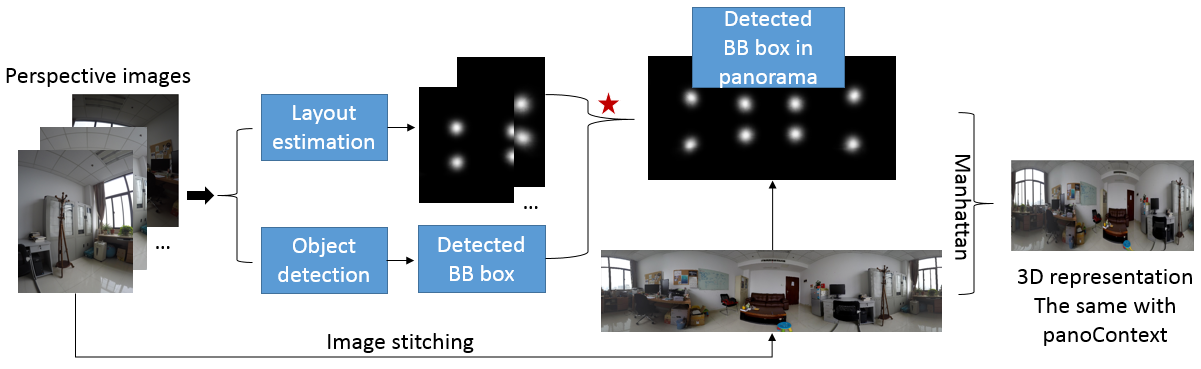
\includegraphics[width=\linewidth]{figs/ppline.png}
	\caption{System overview. }
	\label{fig:overview}
\end{figure*}

\subsection{Single-view room Layout Estimation}
\label{sec:layout}

Many methods have been proposed to estimate the room layout from a single RGB image. 
%In this section, we are going to recover the room layout for perspective images from different views. 
DNN-based techniques of room layout estimation typically represent the room layout as a segmentation of semantic surfaces including walls, ceilings and floors~\cite{Delay, ours} or as the semantic boundaries or intersection points among them \cite{CFILE}. 
A direct way to achieve our goal is to utilize existing methods to estimate the layout for each view, and then combine these representations to produce the complete-room 3D layout. 
However, this method is not efficient due to many redundant predictions caused by overlaps across views. 
To avoid redundant predictions or even to benefit from them, we propose a \emph{secondary representation} of a room layout on perspective images. The room layout under each view is only represented by the intersections of vertical walls and ceiling or floor. We call these intersections secondary keypoints. 
\xj{What about the case when there in only one wall surface?}
Obviously, without the extra intersections of two semantic planes on the image boundaries, we cannot recover the room layout from a single perspective. However, these secondary keypoints in overlapping views are sufficient to reconstruct the 3D layout of the entire room. Compared to previous representations, our secondary keypoints are quite simplified and easier to train. It also naturally avoids a lot of redundant predictions. 

\paragraph{Layout Representation.}
\xj{Explain more details of this new representation: add a figure. and more constraints? say, there are at most four points on each image? Split them to upper/lower parts?}
 
%We use an encoder-decoder Network structure proposed in \cite{RoomNet} to estimate room layouts on perspective images. The room layout is represented by a series of keypoints in a particular order. The keypoints are the intersection of different semantic planes on the the perspective images. By learning the location of these keypoints, a room layout can be reconstructed by simply connect these keypoints in a specific order.

\noindent\textbf{Network Architecture.} We adopt the encoder-decoder architecture proposed by \cite{roomnet} with modifications \xj{since it is an end-to-end framework without any post-processing}. 
Our network for room corner estimation from a single-view image is shown in Fig.~\ref{fig:network}. 
\xj{We mainly make two modifications: decode part and classfication branch.} 
First, the encoder part consists of 13 convolutional layers, which are topologically identical to the VGG16 network. It encodes the $320\times320$ input images to $10\times10$ feature maps. 
We modify the decoder part to upsample the feature maps from the bottleneck layer with low resolution to full input resolution. \xj{what is the original decoder?}
%
Second, we remove the classification branch of the original RoomNet because our simplified representation is consist for different topology of visible surfaces in the scene. 
\xj{Therefore, our network outputs ... ?}
 

\begin{figure}
	\centering
	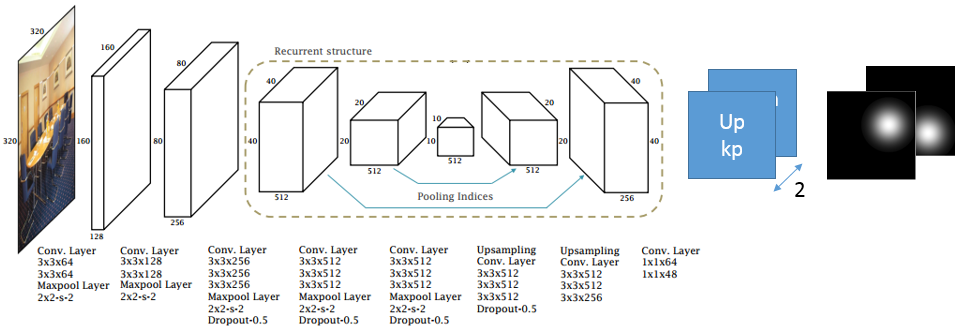
\includegraphics[width=\linewidth]{figs/network.png}
	\caption{Network architecture. }
	\label{fig:network}
\end{figure}

\noindent\textbf{Training.} 
The secondary keypoints can be divided into two categories according to semantics: the intersection of two walls and ceiling or the intersection of two walls and floor.\xj{Move this sentence to the representation paragraph.}

We train the network to regress these two kinds of keypoints separately in order to eliminate the ambiguity between them. For this reason, the output of our network is a $w \times h \times 2$ probability array $T$, where $w$ and $h$ stand for the width and length of the input image. Each of the 2 slices can be viewed as a probability map for the secondary keypoints in a corresponding category. 
We adopt the PanoContext dataset \cite{pano} and relabeled Stanford 2D-3D dataset \cite{layoutnet} to train our layout estimation network. 
To obtain multiple overlapping perspective images, we project the panoramic images into different views using the toolkit provided by \cite{pano}. The ground truth of the secondary keypoints is represented by several 2D Gaussian heatmaps centered at their locations. We adjust the distribution imbalance between foreground and background pixels by degrading the gradient weight of background pixels with a coefficient of 0.2.

%The RoomNet-basic struture in \cite{RoomNet} is adopted in our training stage for efficiency. We first pretrain the Network on LSUN \cite{LSUN2016} training set. Then, to finetune the model on images from different views in the same room, we project the panorama from \cite{PanoContext} to $k$ views. We set $k$ to 12 and 24 in our experiment. The layout ground truth is relabeled using the same projection. 


\subsection{Layout composition}
\label{sec:merging}
In this section, we combine the predicted layouts from different perspectives and generate a panoramic layout estimation. Fisrt, we stitch the input multi-view images into a panoramic image. Then, we use the same mapping to map the predicted probability array $T$ from different views into a panoramic predictions and averaged across views. To reduce the noise caused by false predictions from specific perspectives, we calculate the LOG response of the panoramic predictions at a certain scale (depending on the radius of the keypoints), $\sigma$ is set to 21 in our case. After that, we sum up the probability maps from two channel to get a holistc probability map. Finally, we follow the post-processing method in \cite{LayoutNet} to obtain the locations of the keypoints in the panorama. In brief, the holistic probability map are summed across rows to find four local maxima for columns, then two largest peaks are found along each of the four columns. In this way, we attain the location of eight keypoints for each panorama. Then the whole room layout can be reconstructed by connecting these eight keypoints. 


\comments{
\subsection{Alignment and 3D Reconstruction}
\label{sec:align}

(Optional and undone) In this section, we align the panoramic images to make sure that wall-wall boundaries are vertical to the floor. If we use the panorama to generate testing images, this step can be omitted as the reprojected panoramic images naturally met this alignment condition. Then the aligned panorama can be further rendered into a 3D representation. These two steps are implemented using existing techniques but the rendering part is not yet available. 
}
